\chapter{Shower Generation}\label{sec:GAN}

Generative Adversarial Networks are composed of two networks, a discriminator and a generator. Our model, 3DGAN, implements an architecture inspired by the auxiliary classifier GAN~\cite{acgan}. The generator takes as input a specific particle type, flight direction, and energy, and generates the 3D image of an energy deposit using an auxiliary input vector of random quantities (latent vector). 
The output has the same format as the 3D array of ECAL hits in the GEN sample (see Section~\ref{sec:data}). The discriminator network receives as input an ECAL 3D array and classifies it as {\it real} (coming from the GEANT4-generated GEN dataset) or {\it fake} (produced by the generator).

 Our initial 3DGAN prototype~\cite{NIPS} successfully simulated detector outputs for electrons which were orthogonally incident to the calorimeter surface. In addition, the discriminator performed an auxiliary regression task on the input particle energy. This task was used to cross check the quality of the generation process. 
 
 In this study, we consider a more complex dataset, e.g., due to the variable incident angle of the incoming electron on the inner ECAL surface. To monitor this additional complexity, we include more components in the loss function, related to the regression of the particle direction and the pixel intensity distribution (energy deposition in cells). This will be described in more detail below.

Before training our GAN, we pre-processed the GEN dataset by replacing each cell energy content $E$ with $E^\alpha$, where $\alpha<1$ is a fixed hyperparameter. This pre-processing compensates for the large energy range (about 7 orders of magnitude) covered by individual cell energies, and mitigates some performance degradation we previously observed at low energies. After testing for different values of $\alpha$, we observed optimal performance for $\alpha=0.85$.

\begin{figure*}[htbp]
\centering
    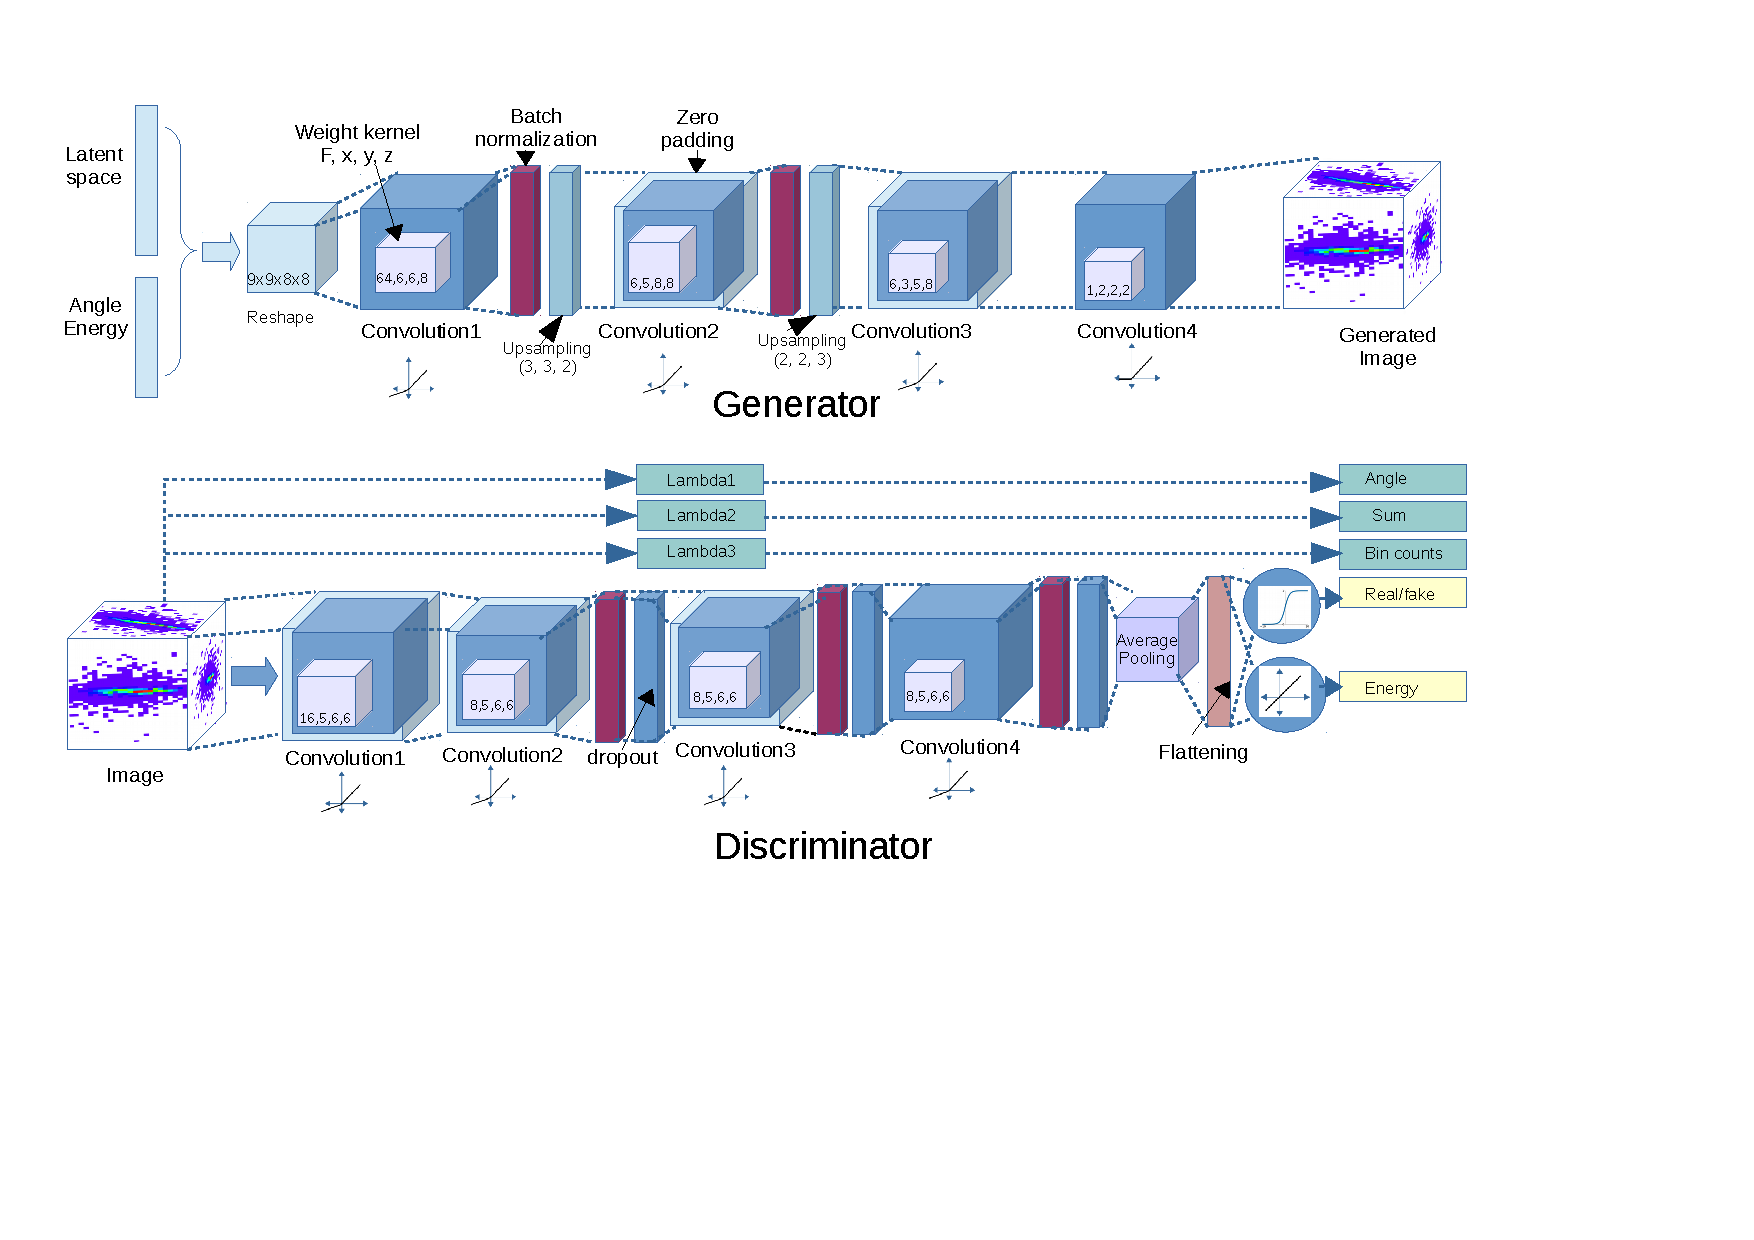
\includegraphics[scale=0.65, trim={0cm 6cm 3.5cm 1.8cm}]{images/gan_model_alt_upsampling.pdf}
    \caption{3DGAN generator and discriminator network architectures}
    \label{fig:GAN_arch}
\end{figure*}

\subsection{GAN Architecture}
\label{sec:GANarch}

The 3DGAN architecture is based on 3-dimensional convolutional layers~\cite{conv}, as shown in Figure~\ref{fig:GAN_arch}. The generator takes as input a vector with a desired particle energy and angle, and concatenates a latent vector of 254 normally distributed random numbers. This goes through a set of alternating upsampling and convolutional layers. The first convolution layer has $64$ filters with $6 \times 6 \times 8$ kernels. The next two convolutional layers have $6$ filters of $5 \times 8 \times 8$ and $3 \times 5 \times 8$ kernels, respectively. The last convolutional layer has a single filter with a $2 \times 2 \times 2$ kernel. The first three layers are activated by leaky ReLU functions~\cite{LeakyReLU}, while ReLU functions~\cite{ReLU} are used for the last layer. Batch normalization~\cite{batchnorm} and upscaling layers were added after the first and second convolutional layers.

The discriminator takes as input a $51  \times 51  \times 25$ array and consists of four 3D convolutional layers. The first layer has $16$ filters with $5 \times 6 \times 6$ kernels. The second, third, and fourth convolutional layers each have $8$ filters with $5 \times 6 \times 6$ kernels. There are leaky ReLU activation functions in each convolutional layer. Batch normalization and dropout~\cite{dropout} layers are added after the second, third, and fourth convolutional layers. The output of the final convolution layer is flattened and connected to two output nodes: a classification node, activated by a sigmoid and returning the probability of a given input to be true or fake; and a regression node, activated by a linear function and returning the input particle energy.
The 3DGAN model is implemented in KERAS~\cite{keras} and Tensorflow~\cite{tensorflow2015-whitepaper}.

Aside from the architecture shown here, we also tested the use of a Wasserstein GAN~\cite{wgan}, but found no practical advantage in terms of computational speed-up or training performance.

\subsection{Training and Results}
The 3DGAN loss function
\begin{equation}
    L_{Tot} = W_{G}L_{G} + W_{P}L_{P} + W_{A}L_{A} + W_{E}L_{E} + W_{B}L_{B} 
\label{eq:loss}
\end{equation}
is built as a weighted sum of several terms: a binary cross entropy ($L_{G}$) function of the real/fake probability returned by the discriminator, mean absolute percentage error terms (MAPE) related to the regression of the primary-particle energy ($L_{P}$) , the total deposited energy ($L_{E}$) and the binned pixel intensity distribution ($L_{B}$), and a mean absolute error (MAE) for the incident angles measurement ($L_{A}$). The binary cross entropy term, percentage errors and absolute error are weighted by $3.0$, $0.1$ and $25$ respectively. The weights $W$ are tuned to balance the relative importance of each contribution. The predicted energy and incident angle provide a feedback on the conditioning of the image. The binned pixel intensity distribution loss compares the counts in different bins of pixel intensities. 

The model training is done using the RMSprop~\cite{rmsProp} optimiser. We alternately train the discriminator on a batch of real images and a batch of generated images, applying label switching. We then train the generator while freezing the discriminator weights.

Figure~\ref{fig:GEANT4_events} shows a few events from the GEN data set. The events were selected to cover both ends of the primary-particle energy and angle spectrum. Figure~\ref{fig:GAN_events} presents the corresponding generated events with the same primary particle energy and angle as the GEN events in Figure~\ref{fig:GEANT4_events}. Initial visual inspection shows no obvious difference between the original and GAN generated images. A detailed validation based on several energy-shape related features confirms these results. We discuss a few examples below.

\begin{figure}[htbp]
    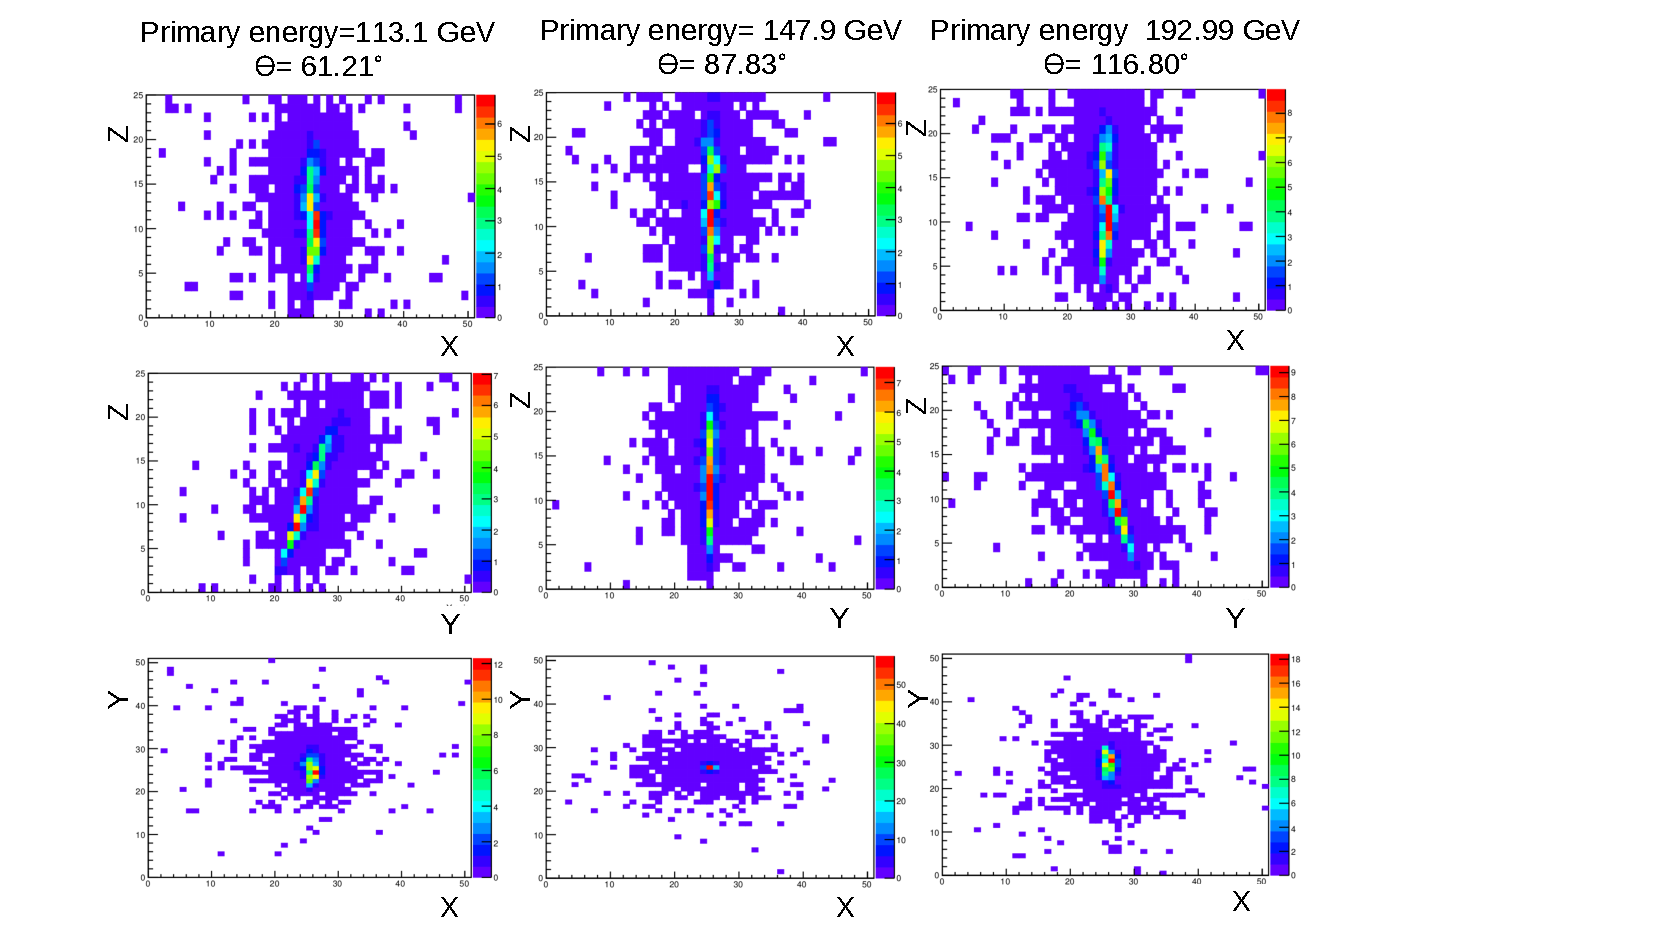
\includegraphics[width=0.48\textwidth]{images/GAN_g4_events.pdf}
    \caption{GEN sample: electrons with different primary particle energies and angles.}
    \label{fig:GEANT4_events}
\end{figure}

\begin{figure}[htbp]
    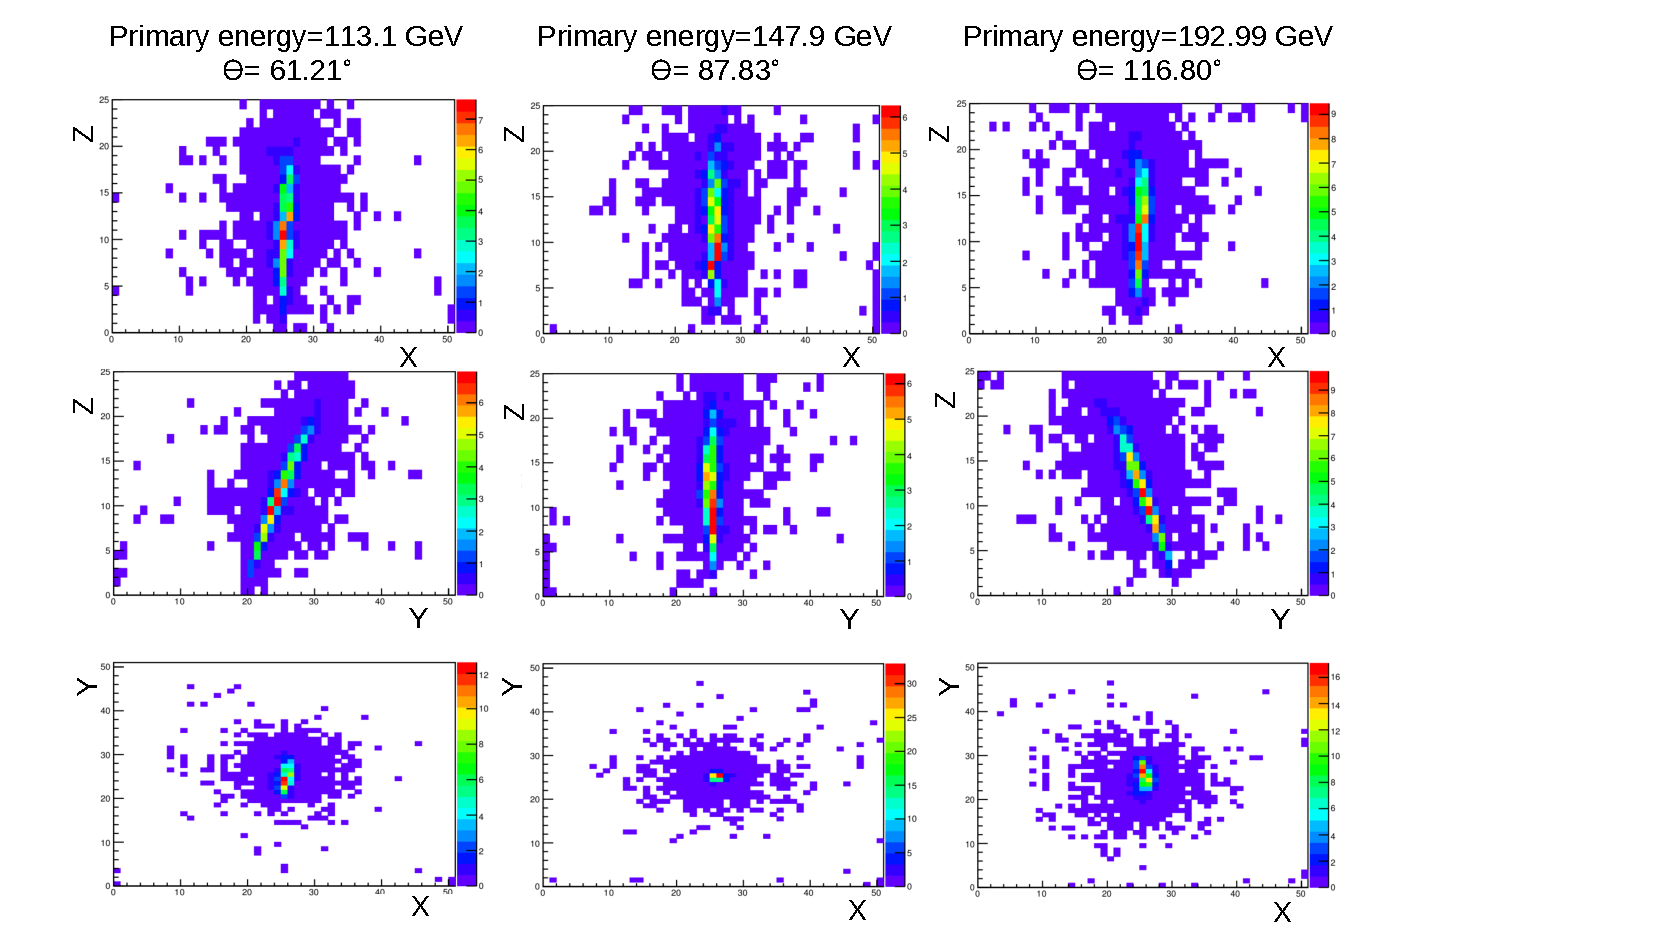
\includegraphics[width=0.48\textwidth]{images/GAN_gan_events.pdf}
    \caption{GAN generated electrons with primary energies and angles corresponding to the electrons showed in Figure~\ref{fig:GEANT4_events}.}
    \label{fig:GAN_events}
\end{figure}

The top row in Figure~\ref{fig:GAN_features1} shows the ratio between the total energy deposited in the calorimeter and the primary particle energy as a function of the primary particle energy (we refer to it as "sampling fraction") for different angle values. 3DGAN can nicely reproduce the expected behaviour over the whole energy spectrum. The second row in Figure~\ref{fig:GAN_features1} shows the number of hits above a $3 \times 10^{-4}$ MeV threshold: the GAN prediction is slightly broader than the Monte Carlo, consistently with the slight overestimation on the shower shapes distributions (\ref{fig:GAN_features2}).  Figure~\ref{fig:GAN_features1} also shows the calorimeter shower shapes projected onto the x, y, and z axes. Here, z is the axis pointing into the calorimeter, perpendicular to its surface. The agreement is very good, and in particular 3DGAN is able to mimic the way the energy distributions changes with incident angle. 
Figure~\ref{fig:GAN_features2} shows some additional features aimed at defining the shape of the deposited energy distribution. In particular the second moments along the x,y and z axes are shown on the first column, measuring the width of the deposited energy distribution along those axes. The second column shows the way the energy is deposited along the depth of the calorimeter, by splitting the calorimeter in three parts along the longitudinal direction and measuring the ratios between the energy deposited in each third  and the total deposited energy. Finally, the third column in Figure~\ref{fig:GAN_features2} highlights the tails of the "energy shapes". It can be seen that, while the core of the distribution is perfectly described by 3DGAN, the network tends to overestimate the amount of energy deposited at the edges of the volume. It should be noted however that energy depositions in those cells are very sparse. 
\iffalse
\begin{figure}
    \centering
    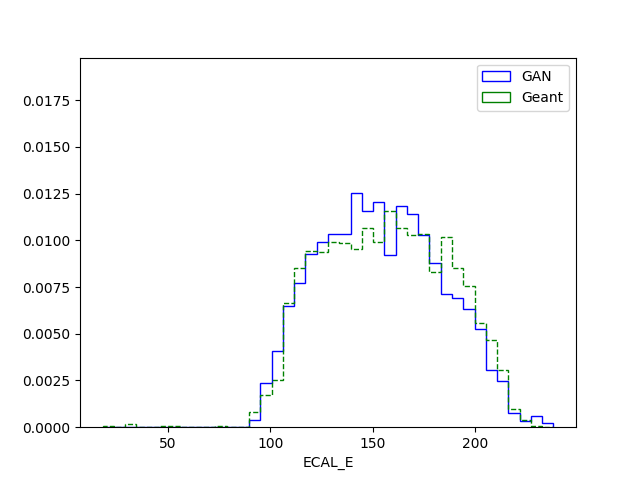
\includegraphics[scale=0.3]{images/GAN_feature_ECAL_E.png}
    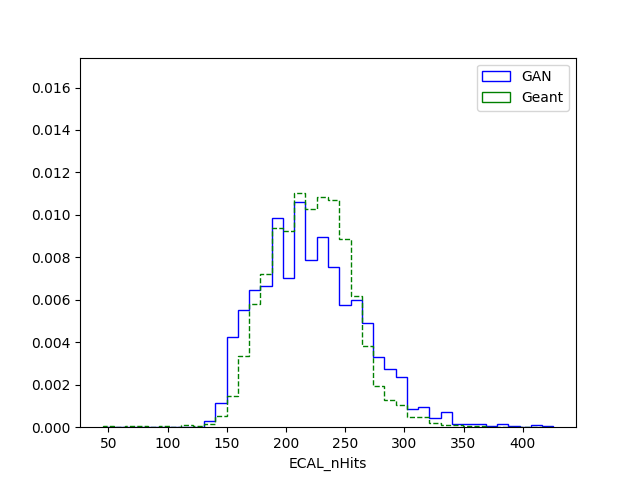
\includegraphics[scale=0.3]{images/GAN_feature_ECAL_nHits.png}
    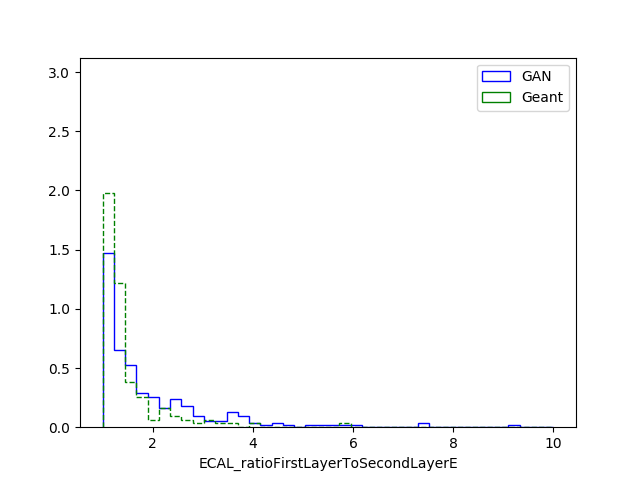
\includegraphics[scale=0.3]{images/GAN_feature_ECAL_ratioFirstLayerToSecondLayerE.png}
    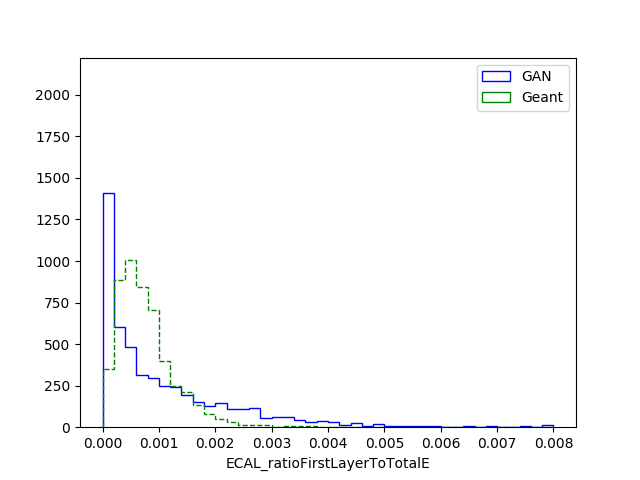
\includegraphics[scale=0.3]{images/GAN_feature_ECAL_ratioFirstLayerToTotalE.png}
    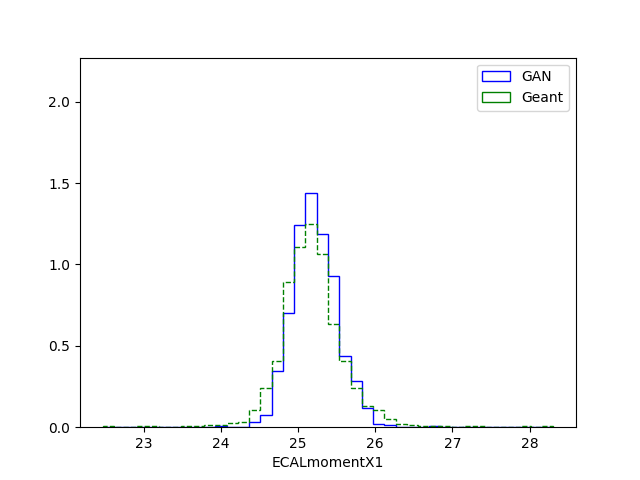
\includegraphics[scale=0.3]{images/GAN_feature_ECALmomentX1.png}
    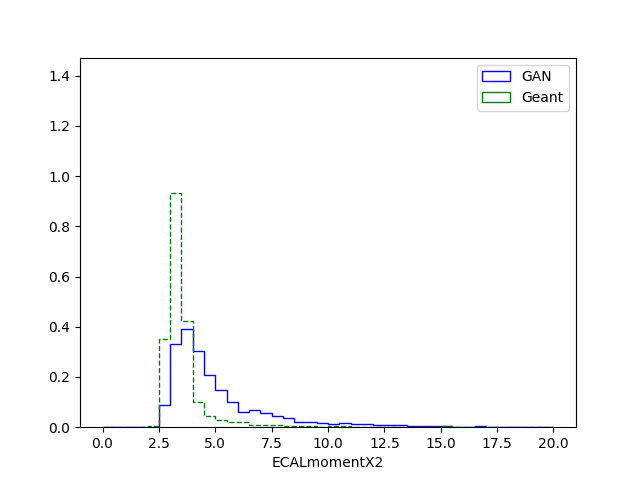
\includegraphics[scale=0.3]{images/GAN_feature_ECALmomentX2.png}
    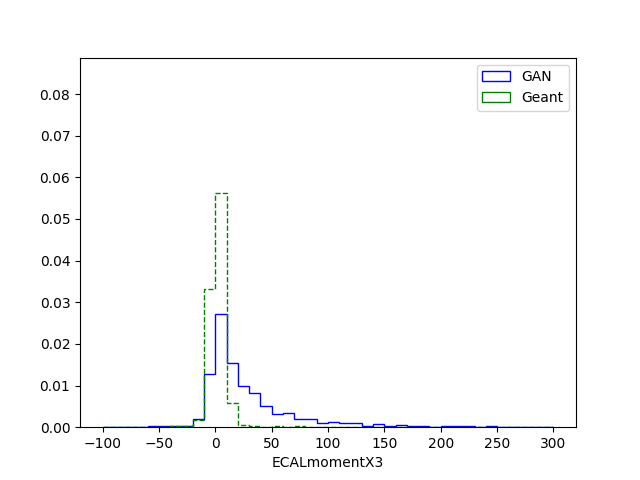
\includegraphics[scale=0.3]{images/GAN_feature_ECALmomentX3.png}
    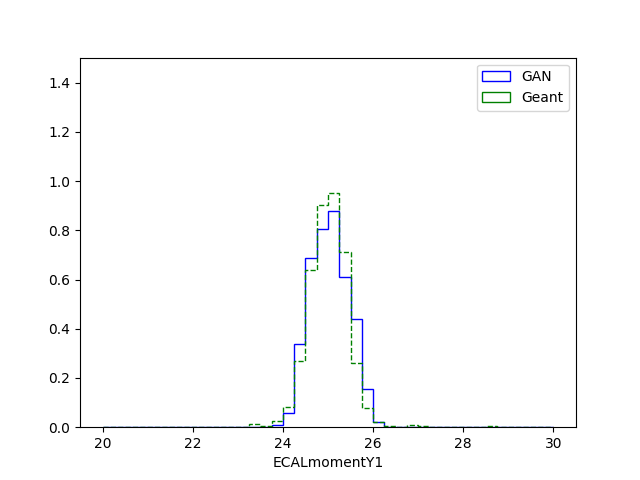
\includegraphics[scale=0.3]{images/GAN_feature_ECALmomentY1.png}
    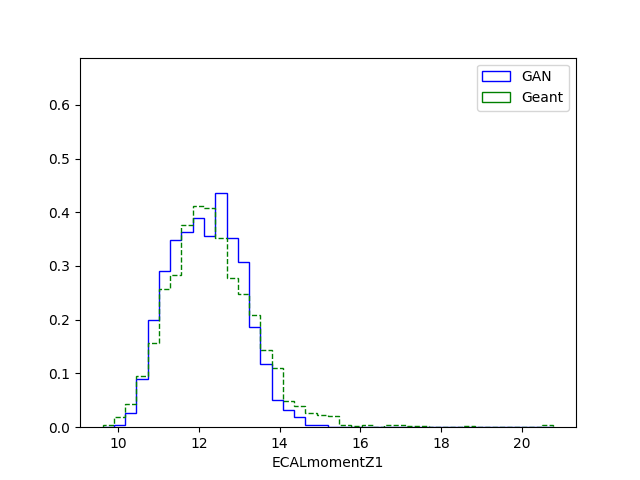
\includegraphics[scale=0.3]{images/GAN_feature_ECALmomentZ1.png}
    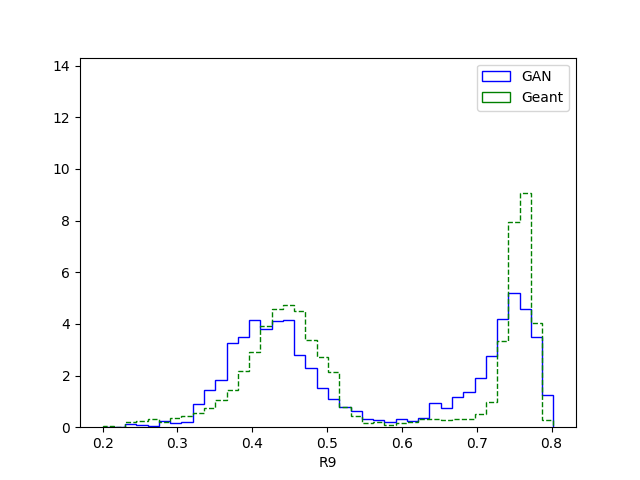
\includegraphics[scale=0.3]{images/GAN_feature_R9.png}
    \caption{GAN vs. GEANT comparisons for various features. {\bf theta should be $\theta$.}
    \label{fig:GAN_features}}
\end{figure}
\fi
\begin{figure}
    \centering
    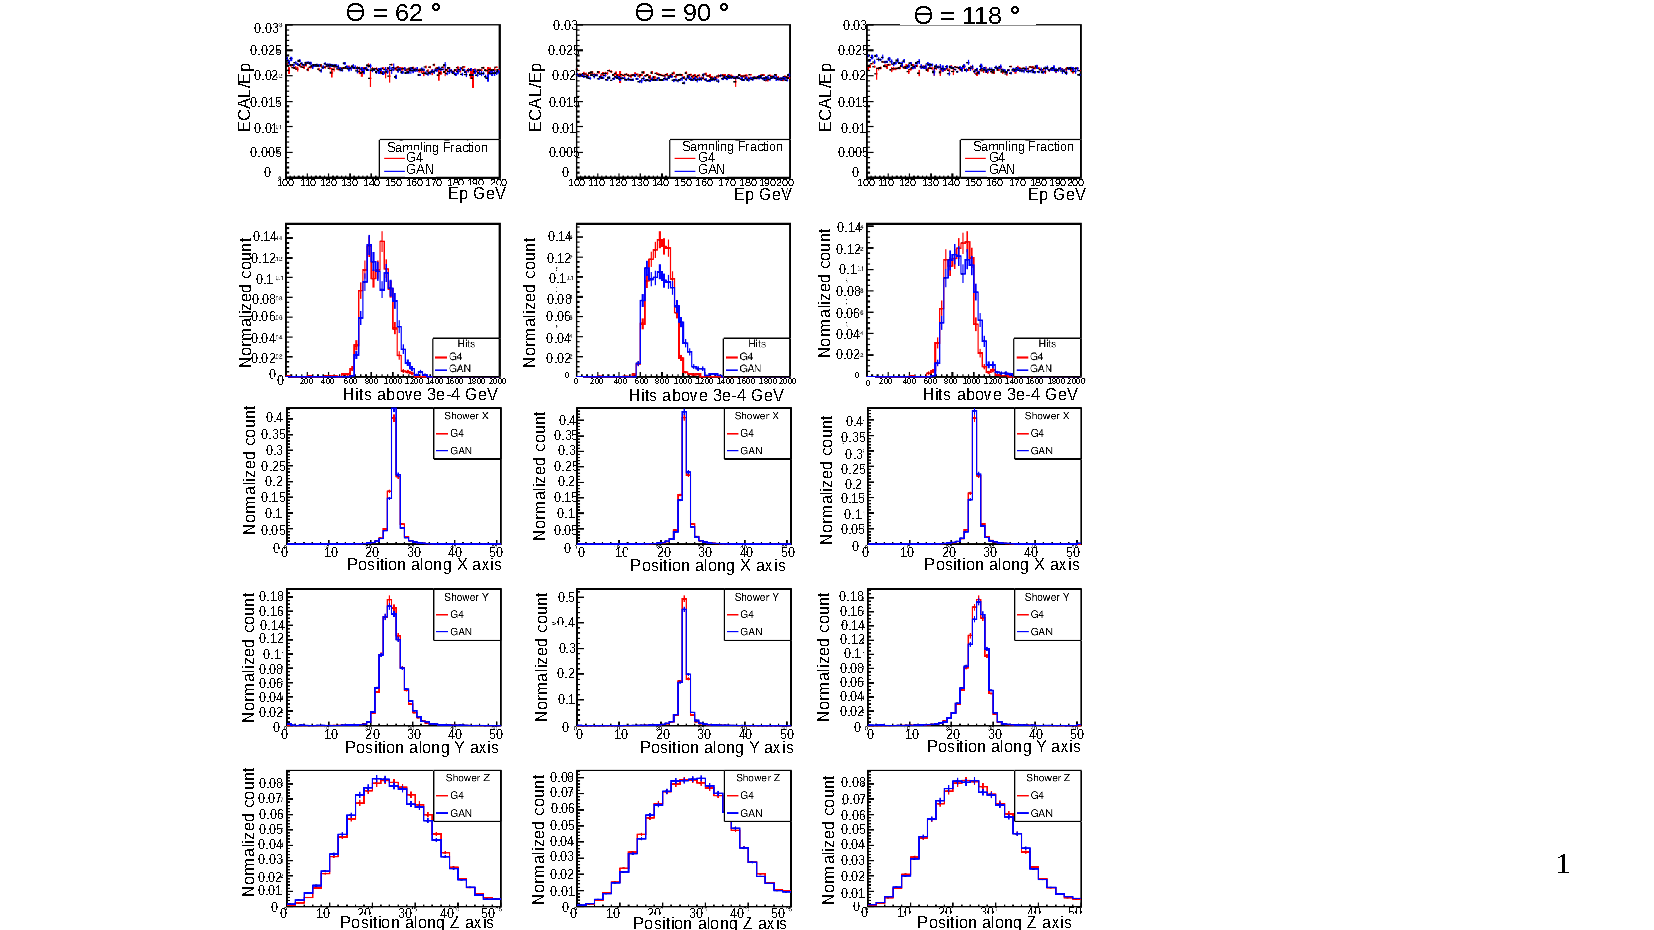
\includegraphics[width=0.48\textwidth, trim={4cm 0cm 9cm 0cm}, clip=true]{images/features_1_rev.pdf}
    \caption{GEANT4 vs. GAN comparison for sampling fraction, number
      of hits and shower shapes along x,y,z axis for different angle
      bins with 100-200 GeV primary particle energies.
      \label{fig:GAN_features1}}
\end{figure}

\begin{figure}
    \centering
    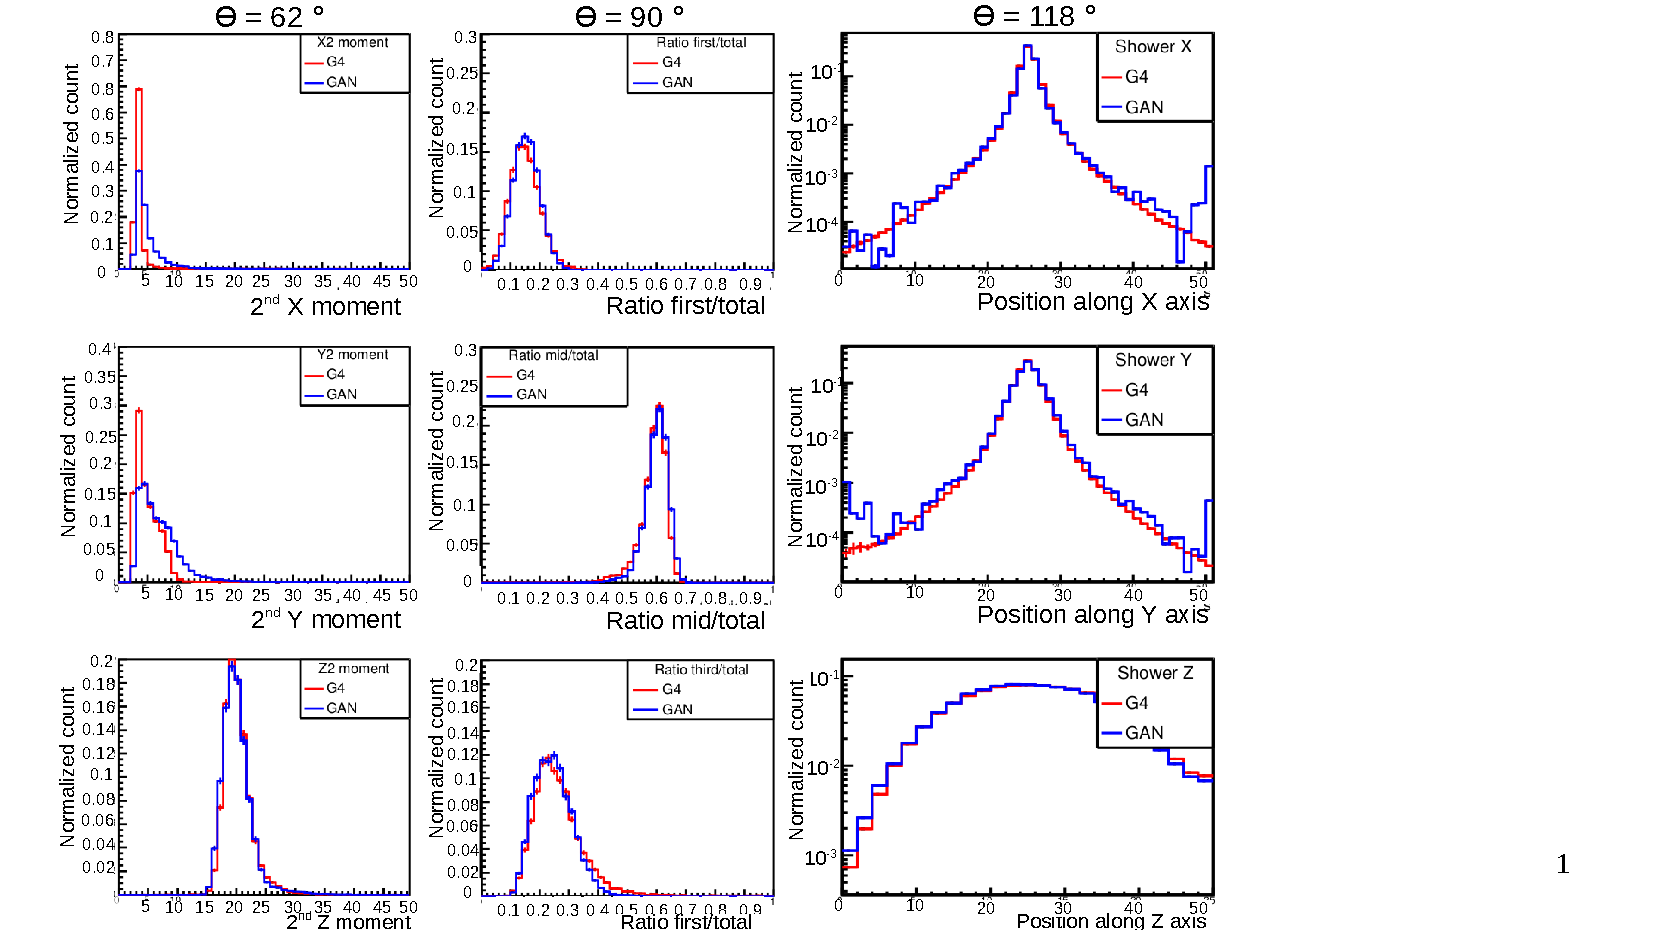
\includegraphics[width=0.48\textwidth, trim={1cm 0cm 7cm 0cm}, clip=true]{images/features_2_rev.pdf}
    \caption{GEANT4 vs. GAN comparison for shower width (second
      moment) in x,y,z, ratio of energy deposited in parts along
      direction of particle traversal to total energy and shower
      shapes along x,y,z axis in log scale for 100-200 GeV primary
      particle energies and 60-120 degrees $\theta$.
      \label{fig:GAN_features2}}
\end{figure}

The 3DGAN training runs in around $1.5$ hours per epoch on a single NVIDIA GeForce GTX 1080 card for $60$ epochs. The simulation  time  on a Intel  Xeon 8180  is about $13$ ms/particle  and it goes down to about $4$ ms/particle on a NVIDIA  GeForce  GTX  1080. For  comparison  GEANT4  simulation takes  about $17$ seconds  per  particle on  a  Intel  Xeon  8180 (currently  it  is  not  possible  to  run a full  GEANT4-based  simulation  on  GPUs). Thus our GAN represents a potential simulation speedup of over 4,000 times for this specific aspect of the event simulation.

When given as input to a particle regression and reconstruction model (see section~\ref{sec:reco}), this dataset produces the same output as the original GEANT4 sample, as described in Appendix~\ref{appendix:RECO_on_GAN}.

\section{End-to-end reconstruction of the ECAL showers produced by the 3DGAN}
\label{appendix:RECO_on_GAN}

\begin{figure}
    \centering
    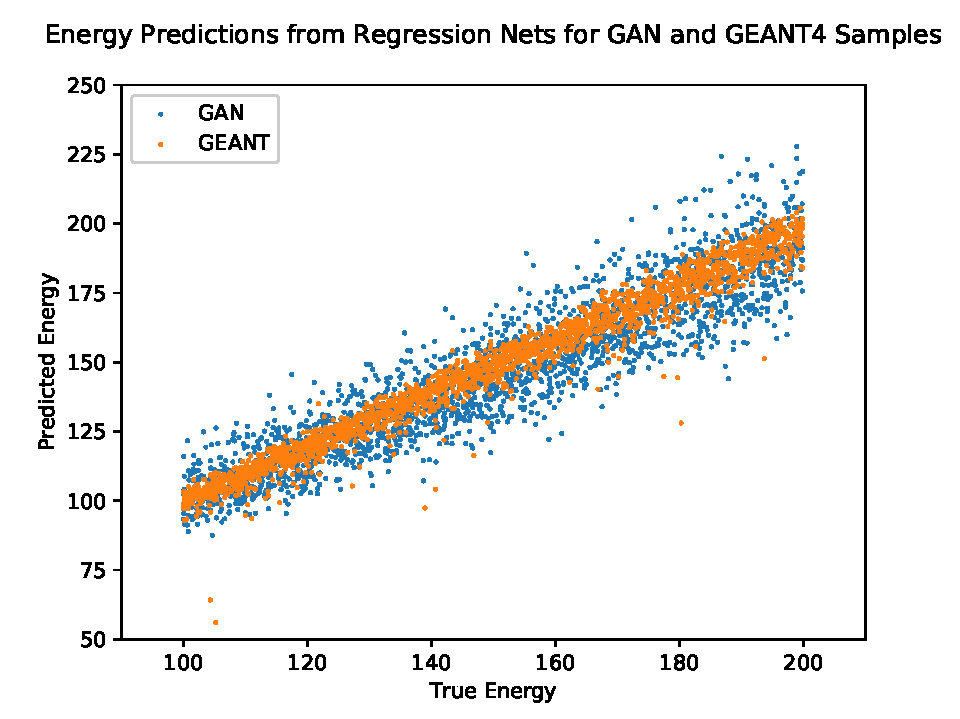
\includegraphics[scale=0.4, trim={0.5cm 0.1cm 0 1.1cm}, clip]{images/GAN_GEANT_energy_regression_comparison.pdf}
    \caption{Predicted vs. true particle energy for GAN and GEANT
      images. Predictions were made using the reconstruction tool described in section~\ref{sec:reco}. This plot was made using 2213 electron events of each type (GAN and GEANT).\label{fig:GAN_regression}}
\end{figure}

\begin{figure}
    \centering
    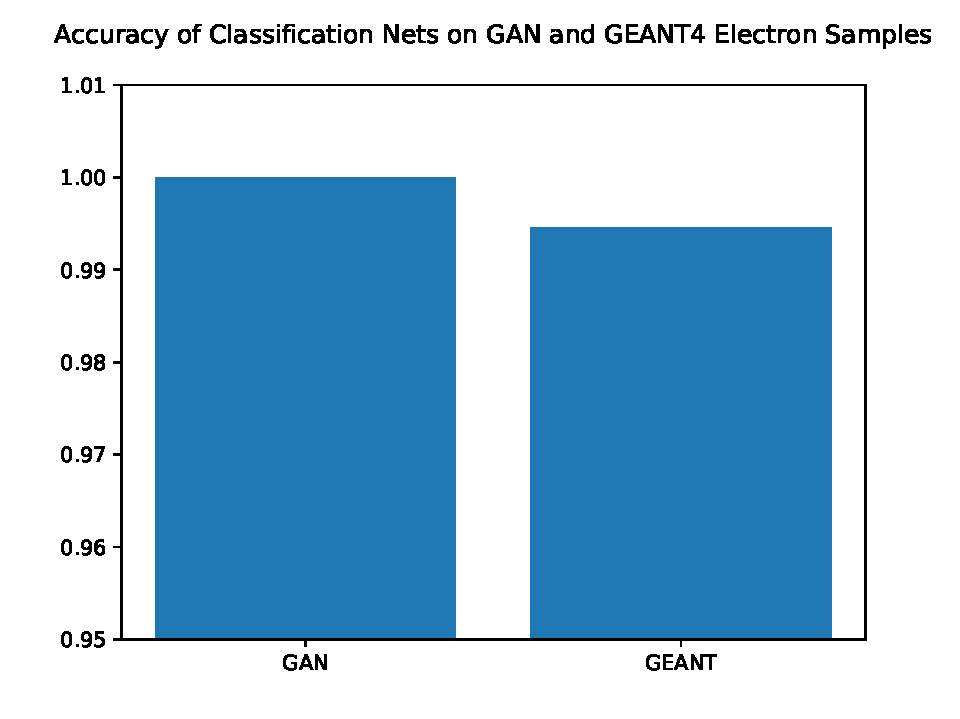
\includegraphics[scale=0.4, trim={0.5cm 0.1cm 0 1.1cm}, clip]{images/GAN_GEANT_class_accuracy_comparison.pdf}
    \caption{Predicted particle type (electron vs. charge pions) for GAN and GEANT images. There were 2213 electron events for each
      type.\label{fig:GAN_classification}}
\end{figure}

In order to further validate the GAN image quality we run the 3D CNN reconstruction network described in section~\ref{sec:reco} on the 3DGAN output and compare the response to the results obtained by running the tool on Monte Carlo data. Figure~\ref{fig:GAN_regression} shows a comparison of the energy resolution obtained on GAN and GEANT4 images. The predicted energy shows a reasonable agreement for the mean while the resolution for GAN images seems to be broader than for GEANT4 images. The classification accuracy presented in Figure~\ref{fig:GAN_classification} is very high (close to $100\%$) for both GAN and GEANT4 events. 